% Wygenerowane przez er.py – nie edytować ręcznie.
\documentclass[tikz,border=4pt]{standalone}
\usepackage[sfdefault]{FiraSans}
\usetikzlibrary{arrows.meta}
\definecolor{head}{HTML}{23373B}
\definecolor{grid}{HTML}{C9CED6}
\definecolor{typ}{HTML}{8A929C}
\definecolor{pk}{HTML}{B7791F}
\definecolor{c-app_user}{HTML}{5B6B7F}
\definecolor{c-student}{HTML}{1F5EFF}
\definecolor{c-lecturer}{HTML}{0B8A7A}
\definecolor{c-section}{HTML}{D9480F}
\definecolor{c-course}{HTML}{2B8A3E}
\definecolor{c-term}{HTML}{7048E8}
\definecolor{c-enrollment}{HTML}{C2255C}
\definecolor{c-room}{HTML}{8D6E63}
\begin{document}
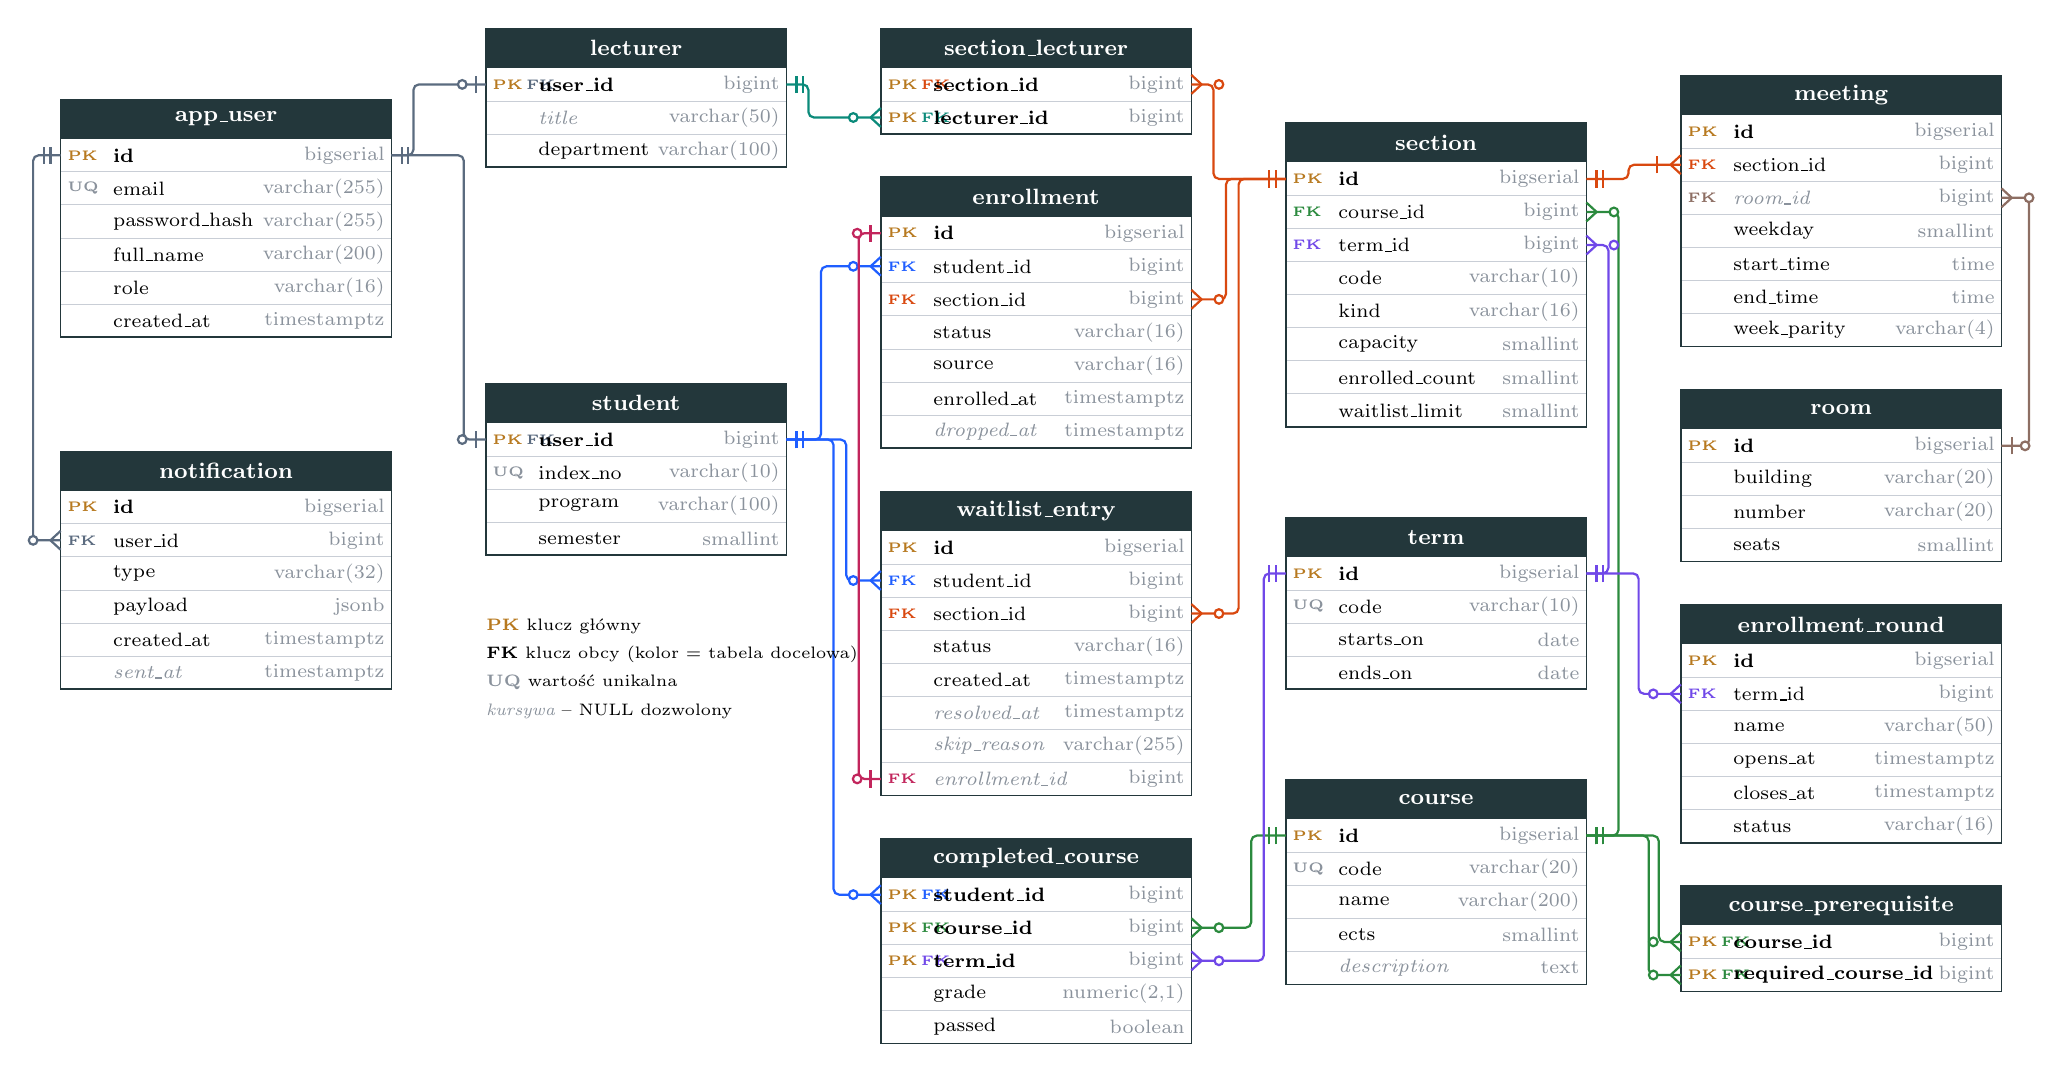
\begin{tikzpicture}[font=\fontsize{7.5}{9}\selectfont]
\fill[white] (0.000,-0.900) rectangle (4.200,-3.920);
\fill[head] (0.000,-0.900) rectangle (4.200,-1.400);
\node[white, font=\fontsize{8}{9}\selectfont\bfseries] at (2.100,-1.150) {app\_user};
\node[anchor=west, inner sep=0, font=\fontsize{5}{6}\selectfont\bfseries] at (0.080,-1.610) {\textcolor{pk}{PK}};
\node[anchor=west, inner sep=0] at (0.660,-1.610) {\textbf{id}};
\node[anchor=east, inner sep=0, text=typ] at (4.120,-1.610) {bigserial};
\draw[grid, line width=0.3pt] (0.000,-1.820) -- (4.200,-1.820);
\node[anchor=west, inner sep=0, font=\fontsize{5}{6}\selectfont\bfseries] at (0.080,-2.030) {\textcolor{typ}{UQ}};
\node[anchor=west, inner sep=0] at (0.660,-2.030) {email};
\node[anchor=east, inner sep=0, text=typ] at (4.120,-2.030) {varchar(255)};
\draw[grid, line width=0.3pt] (0.000,-2.240) -- (4.200,-2.240);
\node[anchor=west, inner sep=0, font=\fontsize{5}{6}\selectfont\bfseries] at (0.080,-2.450) {};
\node[anchor=west, inner sep=0] at (0.660,-2.450) {password\_hash};
\node[anchor=east, inner sep=0, text=typ] at (4.120,-2.450) {varchar(255)};
\draw[grid, line width=0.3pt] (0.000,-2.660) -- (4.200,-2.660);
\node[anchor=west, inner sep=0, font=\fontsize{5}{6}\selectfont\bfseries] at (0.080,-2.870) {};
\node[anchor=west, inner sep=0] at (0.660,-2.870) {full\_name};
\node[anchor=east, inner sep=0, text=typ] at (4.120,-2.870) {varchar(200)};
\draw[grid, line width=0.3pt] (0.000,-3.080) -- (4.200,-3.080);
\node[anchor=west, inner sep=0, font=\fontsize{5}{6}\selectfont\bfseries] at (0.080,-3.290) {};
\node[anchor=west, inner sep=0] at (0.660,-3.290) {role};
\node[anchor=east, inner sep=0, text=typ] at (4.120,-3.290) {varchar(16)};
\draw[grid, line width=0.3pt] (0.000,-3.500) -- (4.200,-3.500);
\node[anchor=west, inner sep=0, font=\fontsize{5}{6}\selectfont\bfseries] at (0.080,-3.710) {};
\node[anchor=west, inner sep=0] at (0.660,-3.710) {created\_at};
\node[anchor=east, inner sep=0, text=typ] at (4.120,-3.710) {timestamptz};
\draw[head, line width=0.6pt] (0.000,-0.900) rectangle (4.200,-3.920);
\fill[white] (0.000,-5.370) rectangle (4.200,-8.390);
\fill[head] (0.000,-5.370) rectangle (4.200,-5.870);
\node[white, font=\fontsize{8}{9}\selectfont\bfseries] at (2.100,-5.620) {notification};
\node[anchor=west, inner sep=0, font=\fontsize{5}{6}\selectfont\bfseries] at (0.080,-6.080) {\textcolor{pk}{PK}};
\node[anchor=west, inner sep=0] at (0.660,-6.080) {\textbf{id}};
\node[anchor=east, inner sep=0, text=typ] at (4.120,-6.080) {bigserial};
\draw[grid, line width=0.3pt] (0.000,-6.290) -- (4.200,-6.290);
\node[anchor=west, inner sep=0, font=\fontsize{5}{6}\selectfont\bfseries] at (0.080,-6.500) {\textcolor{c-app_user}{FK}};
\node[anchor=west, inner sep=0] at (0.660,-6.500) {user\_id};
\node[anchor=east, inner sep=0, text=typ] at (4.120,-6.500) {bigint};
\draw[grid, line width=0.3pt] (0.000,-6.710) -- (4.200,-6.710);
\node[anchor=west, inner sep=0, font=\fontsize{5}{6}\selectfont\bfseries] at (0.080,-6.920) {};
\node[anchor=west, inner sep=0] at (0.660,-6.920) {type};
\node[anchor=east, inner sep=0, text=typ] at (4.120,-6.920) {varchar(32)};
\draw[grid, line width=0.3pt] (0.000,-7.130) -- (4.200,-7.130);
\node[anchor=west, inner sep=0, font=\fontsize{5}{6}\selectfont\bfseries] at (0.080,-7.340) {};
\node[anchor=west, inner sep=0] at (0.660,-7.340) {payload};
\node[anchor=east, inner sep=0, text=typ] at (4.120,-7.340) {jsonb};
\draw[grid, line width=0.3pt] (0.000,-7.550) -- (4.200,-7.550);
\node[anchor=west, inner sep=0, font=\fontsize{5}{6}\selectfont\bfseries] at (0.080,-7.760) {};
\node[anchor=west, inner sep=0] at (0.660,-7.760) {created\_at};
\node[anchor=east, inner sep=0, text=typ] at (4.120,-7.760) {timestamptz};
\draw[grid, line width=0.3pt] (0.000,-7.970) -- (4.200,-7.970);
\node[anchor=west, inner sep=0, font=\fontsize{5}{6}\selectfont\bfseries] at (0.080,-8.180) {};
\node[anchor=west, inner sep=0] at (0.660,-8.180) {\textcolor{typ}{\itshape sent\_at}};
\node[anchor=east, inner sep=0, text=typ] at (4.120,-8.180) {timestamptz};
\draw[head, line width=0.6pt] (0.000,-5.370) rectangle (4.200,-8.390);
\fill[white] (5.400,0.000) rectangle (9.216,-1.760);
\fill[head] (5.400,0.000) rectangle (9.216,-0.500);
\node[white, font=\fontsize{8}{9}\selectfont\bfseries] at (7.308,-0.250) {lecturer};
\node[anchor=west, inner sep=0, font=\fontsize{5}{6}\selectfont\bfseries] at (5.480,-0.710) {\textcolor{pk}{PK}\,\textcolor{c-app_user}{FK}};
\node[anchor=west, inner sep=0] at (6.060,-0.710) {\textbf{user\_id}};
\node[anchor=east, inner sep=0, text=typ] at (9.136,-0.710) {bigint};
\draw[grid, line width=0.3pt] (5.400,-0.920) -- (9.216,-0.920);
\node[anchor=west, inner sep=0, font=\fontsize{5}{6}\selectfont\bfseries] at (5.480,-1.130) {};
\node[anchor=west, inner sep=0] at (6.060,-1.130) {\textcolor{typ}{\itshape title}};
\node[anchor=east, inner sep=0, text=typ] at (9.136,-1.130) {varchar(50)};
\draw[grid, line width=0.3pt] (5.400,-1.340) -- (9.216,-1.340);
\node[anchor=west, inner sep=0, font=\fontsize{5}{6}\selectfont\bfseries] at (5.480,-1.550) {};
\node[anchor=west, inner sep=0] at (6.060,-1.550) {department};
\node[anchor=east, inner sep=0, text=typ] at (9.136,-1.550) {varchar(100)};
\draw[head, line width=0.6pt] (5.400,0.000) rectangle (9.216,-1.760);
\fill[white] (5.400,-4.510) rectangle (9.216,-6.690);
\fill[head] (5.400,-4.510) rectangle (9.216,-5.010);
\node[white, font=\fontsize{8}{9}\selectfont\bfseries] at (7.308,-4.760) {student};
\node[anchor=west, inner sep=0, font=\fontsize{5}{6}\selectfont\bfseries] at (5.480,-5.220) {\textcolor{pk}{PK}\,\textcolor{c-app_user}{FK}};
\node[anchor=west, inner sep=0] at (6.060,-5.220) {\textbf{user\_id}};
\node[anchor=east, inner sep=0, text=typ] at (9.136,-5.220) {bigint};
\draw[grid, line width=0.3pt] (5.400,-5.430) -- (9.216,-5.430);
\node[anchor=west, inner sep=0, font=\fontsize{5}{6}\selectfont\bfseries] at (5.480,-5.640) {\textcolor{typ}{UQ}};
\node[anchor=west, inner sep=0] at (6.060,-5.640) {index\_no};
\node[anchor=east, inner sep=0, text=typ] at (9.136,-5.640) {varchar(10)};
\draw[grid, line width=0.3pt] (5.400,-5.850) -- (9.216,-5.850);
\node[anchor=west, inner sep=0, font=\fontsize{5}{6}\selectfont\bfseries] at (5.480,-6.060) {};
\node[anchor=west, inner sep=0] at (6.060,-6.060) {program};
\node[anchor=east, inner sep=0, text=typ] at (9.136,-6.060) {varchar(100)};
\draw[grid, line width=0.3pt] (5.400,-6.270) -- (9.216,-6.270);
\node[anchor=west, inner sep=0, font=\fontsize{5}{6}\selectfont\bfseries] at (5.480,-6.480) {};
\node[anchor=west, inner sep=0] at (6.060,-6.480) {semester};
\node[anchor=east, inner sep=0, text=typ] at (9.136,-6.480) {smallint};
\draw[head, line width=0.6pt] (5.400,-4.510) rectangle (9.216,-6.690);
\fill[white] (10.416,0.000) rectangle (14.360,-1.340);
\fill[head] (10.416,0.000) rectangle (14.360,-0.500);
\node[white, font=\fontsize{8}{9}\selectfont\bfseries] at (12.388,-0.250) {section\_lecturer};
\node[anchor=west, inner sep=0, font=\fontsize{5}{6}\selectfont\bfseries] at (10.496,-0.710) {\textcolor{pk}{PK}\,\textcolor{c-section}{FK}};
\node[anchor=west, inner sep=0] at (11.076,-0.710) {\textbf{section\_id}};
\node[anchor=east, inner sep=0, text=typ] at (14.280,-0.710) {bigint};
\draw[grid, line width=0.3pt] (10.416,-0.920) -- (14.360,-0.920);
\node[anchor=west, inner sep=0, font=\fontsize{5}{6}\selectfont\bfseries] at (10.496,-1.130) {\textcolor{pk}{PK}\,\textcolor{c-lecturer}{FK}};
\node[anchor=west, inner sep=0] at (11.076,-1.130) {\textbf{lecturer\_id}};
\node[anchor=east, inner sep=0, text=typ] at (14.280,-1.130) {bigint};
\draw[head, line width=0.6pt] (10.416,0.000) rectangle (14.360,-1.340);
\fill[white] (10.416,-1.890) rectangle (14.360,-5.330);
\fill[head] (10.416,-1.890) rectangle (14.360,-2.390);
\node[white, font=\fontsize{8}{9}\selectfont\bfseries] at (12.388,-2.140) {enrollment};
\node[anchor=west, inner sep=0, font=\fontsize{5}{6}\selectfont\bfseries] at (10.496,-2.600) {\textcolor{pk}{PK}};
\node[anchor=west, inner sep=0] at (11.076,-2.600) {\textbf{id}};
\node[anchor=east, inner sep=0, text=typ] at (14.280,-2.600) {bigserial};
\draw[grid, line width=0.3pt] (10.416,-2.810) -- (14.360,-2.810);
\node[anchor=west, inner sep=0, font=\fontsize{5}{6}\selectfont\bfseries] at (10.496,-3.020) {\textcolor{c-student}{FK}};
\node[anchor=west, inner sep=0] at (11.076,-3.020) {student\_id};
\node[anchor=east, inner sep=0, text=typ] at (14.280,-3.020) {bigint};
\draw[grid, line width=0.3pt] (10.416,-3.230) -- (14.360,-3.230);
\node[anchor=west, inner sep=0, font=\fontsize{5}{6}\selectfont\bfseries] at (10.496,-3.440) {\textcolor{c-section}{FK}};
\node[anchor=west, inner sep=0] at (11.076,-3.440) {section\_id};
\node[anchor=east, inner sep=0, text=typ] at (14.280,-3.440) {bigint};
\draw[grid, line width=0.3pt] (10.416,-3.650) -- (14.360,-3.650);
\node[anchor=west, inner sep=0, font=\fontsize{5}{6}\selectfont\bfseries] at (10.496,-3.860) {};
\node[anchor=west, inner sep=0] at (11.076,-3.860) {status};
\node[anchor=east, inner sep=0, text=typ] at (14.280,-3.860) {varchar(16)};
\draw[grid, line width=0.3pt] (10.416,-4.070) -- (14.360,-4.070);
\node[anchor=west, inner sep=0, font=\fontsize{5}{6}\selectfont\bfseries] at (10.496,-4.280) {};
\node[anchor=west, inner sep=0] at (11.076,-4.280) {source};
\node[anchor=east, inner sep=0, text=typ] at (14.280,-4.280) {varchar(16)};
\draw[grid, line width=0.3pt] (10.416,-4.490) -- (14.360,-4.490);
\node[anchor=west, inner sep=0, font=\fontsize{5}{6}\selectfont\bfseries] at (10.496,-4.700) {};
\node[anchor=west, inner sep=0] at (11.076,-4.700) {enrolled\_at};
\node[anchor=east, inner sep=0, text=typ] at (14.280,-4.700) {timestamptz};
\draw[grid, line width=0.3pt] (10.416,-4.910) -- (14.360,-4.910);
\node[anchor=west, inner sep=0, font=\fontsize{5}{6}\selectfont\bfseries] at (10.496,-5.120) {};
\node[anchor=west, inner sep=0] at (11.076,-5.120) {\textcolor{typ}{\itshape dropped\_at}};
\node[anchor=east, inner sep=0, text=typ] at (14.280,-5.120) {timestamptz};
\draw[head, line width=0.6pt] (10.416,-1.890) rectangle (14.360,-5.330);
\fill[white] (10.416,-5.880) rectangle (14.360,-9.740);
\fill[head] (10.416,-5.880) rectangle (14.360,-6.380);
\node[white, font=\fontsize{8}{9}\selectfont\bfseries] at (12.388,-6.130) {waitlist\_entry};
\node[anchor=west, inner sep=0, font=\fontsize{5}{6}\selectfont\bfseries] at (10.496,-6.590) {\textcolor{pk}{PK}};
\node[anchor=west, inner sep=0] at (11.076,-6.590) {\textbf{id}};
\node[anchor=east, inner sep=0, text=typ] at (14.280,-6.590) {bigserial};
\draw[grid, line width=0.3pt] (10.416,-6.800) -- (14.360,-6.800);
\node[anchor=west, inner sep=0, font=\fontsize{5}{6}\selectfont\bfseries] at (10.496,-7.010) {\textcolor{c-student}{FK}};
\node[anchor=west, inner sep=0] at (11.076,-7.010) {student\_id};
\node[anchor=east, inner sep=0, text=typ] at (14.280,-7.010) {bigint};
\draw[grid, line width=0.3pt] (10.416,-7.220) -- (14.360,-7.220);
\node[anchor=west, inner sep=0, font=\fontsize{5}{6}\selectfont\bfseries] at (10.496,-7.430) {\textcolor{c-section}{FK}};
\node[anchor=west, inner sep=0] at (11.076,-7.430) {section\_id};
\node[anchor=east, inner sep=0, text=typ] at (14.280,-7.430) {bigint};
\draw[grid, line width=0.3pt] (10.416,-7.640) -- (14.360,-7.640);
\node[anchor=west, inner sep=0, font=\fontsize{5}{6}\selectfont\bfseries] at (10.496,-7.850) {};
\node[anchor=west, inner sep=0] at (11.076,-7.850) {status};
\node[anchor=east, inner sep=0, text=typ] at (14.280,-7.850) {varchar(16)};
\draw[grid, line width=0.3pt] (10.416,-8.060) -- (14.360,-8.060);
\node[anchor=west, inner sep=0, font=\fontsize{5}{6}\selectfont\bfseries] at (10.496,-8.270) {};
\node[anchor=west, inner sep=0] at (11.076,-8.270) {created\_at};
\node[anchor=east, inner sep=0, text=typ] at (14.280,-8.270) {timestamptz};
\draw[grid, line width=0.3pt] (10.416,-8.480) -- (14.360,-8.480);
\node[anchor=west, inner sep=0, font=\fontsize{5}{6}\selectfont\bfseries] at (10.496,-8.690) {};
\node[anchor=west, inner sep=0] at (11.076,-8.690) {\textcolor{typ}{\itshape resolved\_at}};
\node[anchor=east, inner sep=0, text=typ] at (14.280,-8.690) {timestamptz};
\draw[grid, line width=0.3pt] (10.416,-8.900) -- (14.360,-8.900);
\node[anchor=west, inner sep=0, font=\fontsize{5}{6}\selectfont\bfseries] at (10.496,-9.110) {};
\node[anchor=west, inner sep=0] at (11.076,-9.110) {\textcolor{typ}{\itshape skip\_reason}};
\node[anchor=east, inner sep=0, text=typ] at (14.280,-9.110) {varchar(255)};
\draw[grid, line width=0.3pt] (10.416,-9.320) -- (14.360,-9.320);
\node[anchor=west, inner sep=0, font=\fontsize{5}{6}\selectfont\bfseries] at (10.496,-9.530) {\textcolor{c-enrollment}{FK}};
\node[anchor=west, inner sep=0] at (11.076,-9.530) {\textcolor{typ}{\itshape enrollment\_id}};
\node[anchor=east, inner sep=0, text=typ] at (14.280,-9.530) {bigint};
\draw[head, line width=0.6pt] (10.416,-5.880) rectangle (14.360,-9.740);
\fill[white] (10.416,-10.290) rectangle (14.360,-12.890);
\fill[head] (10.416,-10.290) rectangle (14.360,-10.790);
\node[white, font=\fontsize{8}{9}\selectfont\bfseries] at (12.388,-10.540) {completed\_course};
\node[anchor=west, inner sep=0, font=\fontsize{5}{6}\selectfont\bfseries] at (10.496,-11.000) {\textcolor{pk}{PK}\,\textcolor{c-student}{FK}};
\node[anchor=west, inner sep=0] at (11.076,-11.000) {\textbf{student\_id}};
\node[anchor=east, inner sep=0, text=typ] at (14.280,-11.000) {bigint};
\draw[grid, line width=0.3pt] (10.416,-11.210) -- (14.360,-11.210);
\node[anchor=west, inner sep=0, font=\fontsize{5}{6}\selectfont\bfseries] at (10.496,-11.420) {\textcolor{pk}{PK}\,\textcolor{c-course}{FK}};
\node[anchor=west, inner sep=0] at (11.076,-11.420) {\textbf{course\_id}};
\node[anchor=east, inner sep=0, text=typ] at (14.280,-11.420) {bigint};
\draw[grid, line width=0.3pt] (10.416,-11.630) -- (14.360,-11.630);
\node[anchor=west, inner sep=0, font=\fontsize{5}{6}\selectfont\bfseries] at (10.496,-11.840) {\textcolor{pk}{PK}\,\textcolor{c-term}{FK}};
\node[anchor=west, inner sep=0] at (11.076,-11.840) {\textbf{term\_id}};
\node[anchor=east, inner sep=0, text=typ] at (14.280,-11.840) {bigint};
\draw[grid, line width=0.3pt] (10.416,-12.050) -- (14.360,-12.050);
\node[anchor=west, inner sep=0, font=\fontsize{5}{6}\selectfont\bfseries] at (10.496,-12.260) {};
\node[anchor=west, inner sep=0] at (11.076,-12.260) {grade};
\node[anchor=east, inner sep=0, text=typ] at (14.280,-12.260) {numeric(2,1)};
\draw[grid, line width=0.3pt] (10.416,-12.470) -- (14.360,-12.470);
\node[anchor=west, inner sep=0, font=\fontsize{5}{6}\selectfont\bfseries] at (10.496,-12.680) {};
\node[anchor=west, inner sep=0] at (11.076,-12.680) {passed};
\node[anchor=east, inner sep=0, text=typ] at (14.280,-12.680) {boolean};
\draw[head, line width=0.6pt] (10.416,-10.290) rectangle (14.360,-12.890);
\fill[white] (15.560,-1.200) rectangle (19.376,-5.060);
\fill[head] (15.560,-1.200) rectangle (19.376,-1.700);
\node[white, font=\fontsize{8}{9}\selectfont\bfseries] at (17.468,-1.450) {section};
\node[anchor=west, inner sep=0, font=\fontsize{5}{6}\selectfont\bfseries] at (15.640,-1.910) {\textcolor{pk}{PK}};
\node[anchor=west, inner sep=0] at (16.220,-1.910) {\textbf{id}};
\node[anchor=east, inner sep=0, text=typ] at (19.296,-1.910) {bigserial};
\draw[grid, line width=0.3pt] (15.560,-2.120) -- (19.376,-2.120);
\node[anchor=west, inner sep=0, font=\fontsize{5}{6}\selectfont\bfseries] at (15.640,-2.330) {\textcolor{c-course}{FK}};
\node[anchor=west, inner sep=0] at (16.220,-2.330) {course\_id};
\node[anchor=east, inner sep=0, text=typ] at (19.296,-2.330) {bigint};
\draw[grid, line width=0.3pt] (15.560,-2.540) -- (19.376,-2.540);
\node[anchor=west, inner sep=0, font=\fontsize{5}{6}\selectfont\bfseries] at (15.640,-2.750) {\textcolor{c-term}{FK}};
\node[anchor=west, inner sep=0] at (16.220,-2.750) {term\_id};
\node[anchor=east, inner sep=0, text=typ] at (19.296,-2.750) {bigint};
\draw[grid, line width=0.3pt] (15.560,-2.960) -- (19.376,-2.960);
\node[anchor=west, inner sep=0, font=\fontsize{5}{6}\selectfont\bfseries] at (15.640,-3.170) {};
\node[anchor=west, inner sep=0] at (16.220,-3.170) {code};
\node[anchor=east, inner sep=0, text=typ] at (19.296,-3.170) {varchar(10)};
\draw[grid, line width=0.3pt] (15.560,-3.380) -- (19.376,-3.380);
\node[anchor=west, inner sep=0, font=\fontsize{5}{6}\selectfont\bfseries] at (15.640,-3.590) {};
\node[anchor=west, inner sep=0] at (16.220,-3.590) {kind};
\node[anchor=east, inner sep=0, text=typ] at (19.296,-3.590) {varchar(16)};
\draw[grid, line width=0.3pt] (15.560,-3.800) -- (19.376,-3.800);
\node[anchor=west, inner sep=0, font=\fontsize{5}{6}\selectfont\bfseries] at (15.640,-4.010) {};
\node[anchor=west, inner sep=0] at (16.220,-4.010) {capacity};
\node[anchor=east, inner sep=0, text=typ] at (19.296,-4.010) {smallint};
\draw[grid, line width=0.3pt] (15.560,-4.220) -- (19.376,-4.220);
\node[anchor=west, inner sep=0, font=\fontsize{5}{6}\selectfont\bfseries] at (15.640,-4.430) {};
\node[anchor=west, inner sep=0] at (16.220,-4.430) {enrolled\_count};
\node[anchor=east, inner sep=0, text=typ] at (19.296,-4.430) {smallint};
\draw[grid, line width=0.3pt] (15.560,-4.640) -- (19.376,-4.640);
\node[anchor=west, inner sep=0, font=\fontsize{5}{6}\selectfont\bfseries] at (15.640,-4.850) {};
\node[anchor=west, inner sep=0] at (16.220,-4.850) {waitlist\_limit};
\node[anchor=east, inner sep=0, text=typ] at (19.296,-4.850) {smallint};
\draw[head, line width=0.6pt] (15.560,-1.200) rectangle (19.376,-5.060);
\fill[white] (15.560,-6.210) rectangle (19.376,-8.390);
\fill[head] (15.560,-6.210) rectangle (19.376,-6.710);
\node[white, font=\fontsize{8}{9}\selectfont\bfseries] at (17.468,-6.460) {term};
\node[anchor=west, inner sep=0, font=\fontsize{5}{6}\selectfont\bfseries] at (15.640,-6.920) {\textcolor{pk}{PK}};
\node[anchor=west, inner sep=0] at (16.220,-6.920) {\textbf{id}};
\node[anchor=east, inner sep=0, text=typ] at (19.296,-6.920) {bigserial};
\draw[grid, line width=0.3pt] (15.560,-7.130) -- (19.376,-7.130);
\node[anchor=west, inner sep=0, font=\fontsize{5}{6}\selectfont\bfseries] at (15.640,-7.340) {\textcolor{typ}{UQ}};
\node[anchor=west, inner sep=0] at (16.220,-7.340) {code};
\node[anchor=east, inner sep=0, text=typ] at (19.296,-7.340) {varchar(10)};
\draw[grid, line width=0.3pt] (15.560,-7.550) -- (19.376,-7.550);
\node[anchor=west, inner sep=0, font=\fontsize{5}{6}\selectfont\bfseries] at (15.640,-7.760) {};
\node[anchor=west, inner sep=0] at (16.220,-7.760) {starts\_on};
\node[anchor=east, inner sep=0, text=typ] at (19.296,-7.760) {date};
\draw[grid, line width=0.3pt] (15.560,-7.970) -- (19.376,-7.970);
\node[anchor=west, inner sep=0, font=\fontsize{5}{6}\selectfont\bfseries] at (15.640,-8.180) {};
\node[anchor=west, inner sep=0] at (16.220,-8.180) {ends\_on};
\node[anchor=east, inner sep=0, text=typ] at (19.296,-8.180) {date};
\draw[head, line width=0.6pt] (15.560,-6.210) rectangle (19.376,-8.390);
\fill[white] (15.560,-9.540) rectangle (19.376,-12.140);
\fill[head] (15.560,-9.540) rectangle (19.376,-10.040);
\node[white, font=\fontsize{8}{9}\selectfont\bfseries] at (17.468,-9.790) {course};
\node[anchor=west, inner sep=0, font=\fontsize{5}{6}\selectfont\bfseries] at (15.640,-10.250) {\textcolor{pk}{PK}};
\node[anchor=west, inner sep=0] at (16.220,-10.250) {\textbf{id}};
\node[anchor=east, inner sep=0, text=typ] at (19.296,-10.250) {bigserial};
\draw[grid, line width=0.3pt] (15.560,-10.460) -- (19.376,-10.460);
\node[anchor=west, inner sep=0, font=\fontsize{5}{6}\selectfont\bfseries] at (15.640,-10.670) {\textcolor{typ}{UQ}};
\node[anchor=west, inner sep=0] at (16.220,-10.670) {code};
\node[anchor=east, inner sep=0, text=typ] at (19.296,-10.670) {varchar(20)};
\draw[grid, line width=0.3pt] (15.560,-10.880) -- (19.376,-10.880);
\node[anchor=west, inner sep=0, font=\fontsize{5}{6}\selectfont\bfseries] at (15.640,-11.090) {};
\node[anchor=west, inner sep=0] at (16.220,-11.090) {name};
\node[anchor=east, inner sep=0, text=typ] at (19.296,-11.090) {varchar(200)};
\draw[grid, line width=0.3pt] (15.560,-11.300) -- (19.376,-11.300);
\node[anchor=west, inner sep=0, font=\fontsize{5}{6}\selectfont\bfseries] at (15.640,-11.510) {};
\node[anchor=west, inner sep=0] at (16.220,-11.510) {ects};
\node[anchor=east, inner sep=0, text=typ] at (19.296,-11.510) {smallint};
\draw[grid, line width=0.3pt] (15.560,-11.720) -- (19.376,-11.720);
\node[anchor=west, inner sep=0, font=\fontsize{5}{6}\selectfont\bfseries] at (15.640,-11.930) {};
\node[anchor=west, inner sep=0] at (16.220,-11.930) {\textcolor{typ}{\itshape description}};
\node[anchor=east, inner sep=0, text=typ] at (19.296,-11.930) {text};
\draw[head, line width=0.6pt] (15.560,-9.540) rectangle (19.376,-12.140);
\fill[white] (20.576,-0.600) rectangle (24.648,-4.040);
\fill[head] (20.576,-0.600) rectangle (24.648,-1.100);
\node[white, font=\fontsize{8}{9}\selectfont\bfseries] at (22.612,-0.850) {meeting};
\node[anchor=west, inner sep=0, font=\fontsize{5}{6}\selectfont\bfseries] at (20.656,-1.310) {\textcolor{pk}{PK}};
\node[anchor=west, inner sep=0] at (21.236,-1.310) {\textbf{id}};
\node[anchor=east, inner sep=0, text=typ] at (24.568,-1.310) {bigserial};
\draw[grid, line width=0.3pt] (20.576,-1.520) -- (24.648,-1.520);
\node[anchor=west, inner sep=0, font=\fontsize{5}{6}\selectfont\bfseries] at (20.656,-1.730) {\textcolor{c-section}{FK}};
\node[anchor=west, inner sep=0] at (21.236,-1.730) {section\_id};
\node[anchor=east, inner sep=0, text=typ] at (24.568,-1.730) {bigint};
\draw[grid, line width=0.3pt] (20.576,-1.940) -- (24.648,-1.940);
\node[anchor=west, inner sep=0, font=\fontsize{5}{6}\selectfont\bfseries] at (20.656,-2.150) {\textcolor{c-room}{FK}};
\node[anchor=west, inner sep=0] at (21.236,-2.150) {\textcolor{typ}{\itshape room\_id}};
\node[anchor=east, inner sep=0, text=typ] at (24.568,-2.150) {bigint};
\draw[grid, line width=0.3pt] (20.576,-2.360) -- (24.648,-2.360);
\node[anchor=west, inner sep=0, font=\fontsize{5}{6}\selectfont\bfseries] at (20.656,-2.570) {};
\node[anchor=west, inner sep=0] at (21.236,-2.570) {weekday};
\node[anchor=east, inner sep=0, text=typ] at (24.568,-2.570) {smallint};
\draw[grid, line width=0.3pt] (20.576,-2.780) -- (24.648,-2.780);
\node[anchor=west, inner sep=0, font=\fontsize{5}{6}\selectfont\bfseries] at (20.656,-2.990) {};
\node[anchor=west, inner sep=0] at (21.236,-2.990) {start\_time};
\node[anchor=east, inner sep=0, text=typ] at (24.568,-2.990) {time};
\draw[grid, line width=0.3pt] (20.576,-3.200) -- (24.648,-3.200);
\node[anchor=west, inner sep=0, font=\fontsize{5}{6}\selectfont\bfseries] at (20.656,-3.410) {};
\node[anchor=west, inner sep=0] at (21.236,-3.410) {end\_time};
\node[anchor=east, inner sep=0, text=typ] at (24.568,-3.410) {time};
\draw[grid, line width=0.3pt] (20.576,-3.620) -- (24.648,-3.620);
\node[anchor=west, inner sep=0, font=\fontsize{5}{6}\selectfont\bfseries] at (20.656,-3.830) {};
\node[anchor=west, inner sep=0] at (21.236,-3.830) {week\_parity};
\node[anchor=east, inner sep=0, text=typ] at (24.568,-3.830) {varchar(4)};
\draw[head, line width=0.6pt] (20.576,-0.600) rectangle (24.648,-4.040);
\fill[white] (20.576,-4.590) rectangle (24.648,-6.770);
\fill[head] (20.576,-4.590) rectangle (24.648,-5.090);
\node[white, font=\fontsize{8}{9}\selectfont\bfseries] at (22.612,-4.840) {room};
\node[anchor=west, inner sep=0, font=\fontsize{5}{6}\selectfont\bfseries] at (20.656,-5.300) {\textcolor{pk}{PK}};
\node[anchor=west, inner sep=0] at (21.236,-5.300) {\textbf{id}};
\node[anchor=east, inner sep=0, text=typ] at (24.568,-5.300) {bigserial};
\draw[grid, line width=0.3pt] (20.576,-5.510) -- (24.648,-5.510);
\node[anchor=west, inner sep=0, font=\fontsize{5}{6}\selectfont\bfseries] at (20.656,-5.720) {};
\node[anchor=west, inner sep=0] at (21.236,-5.720) {building};
\node[anchor=east, inner sep=0, text=typ] at (24.568,-5.720) {varchar(20)};
\draw[grid, line width=0.3pt] (20.576,-5.930) -- (24.648,-5.930);
\node[anchor=west, inner sep=0, font=\fontsize{5}{6}\selectfont\bfseries] at (20.656,-6.140) {};
\node[anchor=west, inner sep=0] at (21.236,-6.140) {number};
\node[anchor=east, inner sep=0, text=typ] at (24.568,-6.140) {varchar(20)};
\draw[grid, line width=0.3pt] (20.576,-6.350) -- (24.648,-6.350);
\node[anchor=west, inner sep=0, font=\fontsize{5}{6}\selectfont\bfseries] at (20.656,-6.560) {};
\node[anchor=west, inner sep=0] at (21.236,-6.560) {seats};
\node[anchor=east, inner sep=0, text=typ] at (24.568,-6.560) {smallint};
\draw[head, line width=0.6pt] (20.576,-4.590) rectangle (24.648,-6.770);
\fill[white] (20.576,-7.320) rectangle (24.648,-10.340);
\fill[head] (20.576,-7.320) rectangle (24.648,-7.820);
\node[white, font=\fontsize{8}{9}\selectfont\bfseries] at (22.612,-7.570) {enrollment\_round};
\node[anchor=west, inner sep=0, font=\fontsize{5}{6}\selectfont\bfseries] at (20.656,-8.030) {\textcolor{pk}{PK}};
\node[anchor=west, inner sep=0] at (21.236,-8.030) {\textbf{id}};
\node[anchor=east, inner sep=0, text=typ] at (24.568,-8.030) {bigserial};
\draw[grid, line width=0.3pt] (20.576,-8.240) -- (24.648,-8.240);
\node[anchor=west, inner sep=0, font=\fontsize{5}{6}\selectfont\bfseries] at (20.656,-8.450) {\textcolor{c-term}{FK}};
\node[anchor=west, inner sep=0] at (21.236,-8.450) {term\_id};
\node[anchor=east, inner sep=0, text=typ] at (24.568,-8.450) {bigint};
\draw[grid, line width=0.3pt] (20.576,-8.660) -- (24.648,-8.660);
\node[anchor=west, inner sep=0, font=\fontsize{5}{6}\selectfont\bfseries] at (20.656,-8.870) {};
\node[anchor=west, inner sep=0] at (21.236,-8.870) {name};
\node[anchor=east, inner sep=0, text=typ] at (24.568,-8.870) {varchar(50)};
\draw[grid, line width=0.3pt] (20.576,-9.080) -- (24.648,-9.080);
\node[anchor=west, inner sep=0, font=\fontsize{5}{6}\selectfont\bfseries] at (20.656,-9.290) {};
\node[anchor=west, inner sep=0] at (21.236,-9.290) {opens\_at};
\node[anchor=east, inner sep=0, text=typ] at (24.568,-9.290) {timestamptz};
\draw[grid, line width=0.3pt] (20.576,-9.500) -- (24.648,-9.500);
\node[anchor=west, inner sep=0, font=\fontsize{5}{6}\selectfont\bfseries] at (20.656,-9.710) {};
\node[anchor=west, inner sep=0] at (21.236,-9.710) {closes\_at};
\node[anchor=east, inner sep=0, text=typ] at (24.568,-9.710) {timestamptz};
\draw[grid, line width=0.3pt] (20.576,-9.920) -- (24.648,-9.920);
\node[anchor=west, inner sep=0, font=\fontsize{5}{6}\selectfont\bfseries] at (20.656,-10.130) {};
\node[anchor=west, inner sep=0] at (21.236,-10.130) {status};
\node[anchor=east, inner sep=0, text=typ] at (24.568,-10.130) {varchar(16)};
\draw[head, line width=0.6pt] (20.576,-7.320) rectangle (24.648,-10.340);
\fill[white] (20.576,-10.890) rectangle (24.648,-12.230);
\fill[head] (20.576,-10.890) rectangle (24.648,-11.390);
\node[white, font=\fontsize{8}{9}\selectfont\bfseries] at (22.612,-11.140) {course\_prerequisite};
\node[anchor=west, inner sep=0, font=\fontsize{5}{6}\selectfont\bfseries] at (20.656,-11.600) {\textcolor{pk}{PK}\,\textcolor{c-course}{FK}};
\node[anchor=west, inner sep=0] at (21.236,-11.600) {\textbf{course\_id}};
\node[anchor=east, inner sep=0, text=typ] at (24.568,-11.600) {bigint};
\draw[grid, line width=0.3pt] (20.576,-11.810) -- (24.648,-11.810);
\node[anchor=west, inner sep=0, font=\fontsize{5}{6}\selectfont\bfseries] at (20.656,-12.020) {\textcolor{pk}{PK}\,\textcolor{c-course}{FK}};
\node[anchor=west, inner sep=0] at (21.236,-12.020) {\textbf{required\_course\_id}};
\node[anchor=east, inner sep=0, text=typ] at (24.568,-12.020) {bigint};
\draw[head, line width=0.6pt] (20.576,-10.890) rectangle (24.648,-12.230);
\draw[c-app_user, line width=0.8pt, rounded corners=2pt] (0.000,-6.500) -- (-0.350,-6.500) -- (-0.350,-1.610) -- (0.000,-1.610);
\draw[c-app_user, line width=0.8pt] (-0.130,-6.500) -- (0.000,-6.380) (-0.130,-6.500) -- (0.000,-6.620);
\draw[c-app_user, line width=0.8pt, fill=white] (-0.350,-6.500) circle (0.055);
\draw[c-app_user, line width=0.8pt] (-0.130,-1.720) -- (-0.130,-1.500);
\draw[c-app_user, line width=0.8pt] (-0.210,-1.720) -- (-0.210,-1.500);
\draw[c-app_user, line width=0.8pt, rounded corners=2pt] (5.400,-0.710) -- (4.480,-0.710) -- (4.480,-1.610) -- (4.200,-1.610);
\draw[c-app_user, line width=0.8pt] (5.270,-0.820) -- (5.270,-0.600);
\draw[c-app_user, line width=0.8pt, fill=white] (5.100,-0.710) circle (0.055);
\draw[c-app_user, line width=0.8pt] (4.330,-1.720) -- (4.330,-1.500);
\draw[c-app_user, line width=0.8pt] (4.410,-1.720) -- (4.410,-1.500);
\draw[c-app_user, line width=0.8pt, rounded corners=2pt] (5.400,-5.220) -- (5.120,-5.220) -- (5.120,-1.610) -- (4.200,-1.610);
\draw[c-app_user, line width=0.8pt] (5.270,-5.330) -- (5.270,-5.110);
\draw[c-app_user, line width=0.8pt, fill=white] (5.100,-5.220) circle (0.055);
\draw[c-app_user, line width=0.8pt] (4.330,-1.720) -- (4.330,-1.500);
\draw[c-app_user, line width=0.8pt] (4.410,-1.720) -- (4.410,-1.500);
\draw[c-lecturer, line width=0.8pt, rounded corners=2pt] (10.416,-1.130) -- (9.496,-1.130) -- (9.496,-0.710) -- (9.216,-0.710);
\draw[c-lecturer, line width=0.8pt] (10.286,-1.130) -- (10.416,-1.010) (10.286,-1.130) -- (10.416,-1.250);
\draw[c-lecturer, line width=0.8pt, fill=white] (10.066,-1.130) circle (0.055);
\draw[c-lecturer, line width=0.8pt] (9.346,-0.820) -- (9.346,-0.600);
\draw[c-lecturer, line width=0.8pt] (9.426,-0.820) -- (9.426,-0.600);
\draw[c-student, line width=0.8pt, rounded corners=2pt] (10.416,-3.020) -- (9.656,-3.020) -- (9.656,-5.220) -- (9.216,-5.220);
\draw[c-student, line width=0.8pt] (10.286,-3.020) -- (10.416,-2.900) (10.286,-3.020) -- (10.416,-3.140);
\draw[c-student, line width=0.8pt, fill=white] (10.066,-3.020) circle (0.055);
\draw[c-student, line width=0.8pt] (9.346,-5.330) -- (9.346,-5.110);
\draw[c-student, line width=0.8pt] (9.426,-5.330) -- (9.426,-5.110);
\draw[c-student, line width=0.8pt, rounded corners=2pt] (10.416,-7.010) -- (9.976,-7.010) -- (9.976,-5.220) -- (9.216,-5.220);
\draw[c-student, line width=0.8pt] (10.286,-7.010) -- (10.416,-6.890) (10.286,-7.010) -- (10.416,-7.130);
\draw[c-student, line width=0.8pt, fill=white] (10.066,-7.010) circle (0.055);
\draw[c-student, line width=0.8pt] (9.346,-5.330) -- (9.346,-5.110);
\draw[c-student, line width=0.8pt] (9.426,-5.330) -- (9.426,-5.110);
\draw[c-student, line width=0.8pt, rounded corners=2pt] (10.416,-11.000) -- (9.816,-11.000) -- (9.816,-5.220) -- (9.216,-5.220);
\draw[c-student, line width=0.8pt] (10.286,-11.000) -- (10.416,-10.880) (10.286,-11.000) -- (10.416,-11.120);
\draw[c-student, line width=0.8pt, fill=white] (10.066,-11.000) circle (0.055);
\draw[c-student, line width=0.8pt] (9.346,-5.330) -- (9.346,-5.110);
\draw[c-student, line width=0.8pt] (9.426,-5.330) -- (9.426,-5.110);
\draw[c-enrollment, line width=0.8pt, rounded corners=2pt] (10.416,-9.530) -- (10.136,-9.530) -- (10.136,-2.600) -- (10.416,-2.600);
\draw[c-enrollment, line width=0.8pt] (10.286,-9.640) -- (10.286,-9.420);
\draw[c-enrollment, line width=0.8pt, fill=white] (10.116,-9.530) circle (0.055);
\draw[c-enrollment, line width=0.8pt] (10.286,-2.710) -- (10.286,-2.490);
\draw[c-enrollment, line width=0.8pt, fill=white] (10.116,-2.600) circle (0.055);
\draw[c-section, line width=0.8pt, rounded corners=2pt] (14.360,-0.710) -- (14.640,-0.710) -- (14.640,-1.910) -- (15.560,-1.910);
\draw[c-section, line width=0.8pt] (14.490,-0.710) -- (14.360,-0.590) (14.490,-0.710) -- (14.360,-0.830);
\draw[c-section, line width=0.8pt, fill=white] (14.710,-0.710) circle (0.055);
\draw[c-section, line width=0.8pt] (15.430,-2.020) -- (15.430,-1.800);
\draw[c-section, line width=0.8pt] (15.350,-2.020) -- (15.350,-1.800);
\draw[c-section, line width=0.8pt, rounded corners=2pt] (14.360,-3.440) -- (14.800,-3.440) -- (14.800,-1.910) -- (15.560,-1.910);
\draw[c-section, line width=0.8pt] (14.490,-3.440) -- (14.360,-3.320) (14.490,-3.440) -- (14.360,-3.560);
\draw[c-section, line width=0.8pt, fill=white] (14.710,-3.440) circle (0.055);
\draw[c-section, line width=0.8pt] (15.430,-2.020) -- (15.430,-1.800);
\draw[c-section, line width=0.8pt] (15.350,-2.020) -- (15.350,-1.800);
\draw[c-section, line width=0.8pt, rounded corners=2pt] (14.360,-7.430) -- (14.960,-7.430) -- (14.960,-1.910) -- (15.560,-1.910);
\draw[c-section, line width=0.8pt] (14.490,-7.430) -- (14.360,-7.310) (14.490,-7.430) -- (14.360,-7.550);
\draw[c-section, line width=0.8pt, fill=white] (14.710,-7.430) circle (0.055);
\draw[c-section, line width=0.8pt] (15.430,-2.020) -- (15.430,-1.800);
\draw[c-section, line width=0.8pt] (15.350,-2.020) -- (15.350,-1.800);
\draw[c-course, line width=0.8pt, rounded corners=2pt] (14.360,-11.420) -- (15.120,-11.420) -- (15.120,-10.250) -- (15.560,-10.250);
\draw[c-course, line width=0.8pt] (14.490,-11.420) -- (14.360,-11.300) (14.490,-11.420) -- (14.360,-11.540);
\draw[c-course, line width=0.8pt, fill=white] (14.710,-11.420) circle (0.055);
\draw[c-course, line width=0.8pt] (15.430,-10.360) -- (15.430,-10.140);
\draw[c-course, line width=0.8pt] (15.350,-10.360) -- (15.350,-10.140);
\draw[c-term, line width=0.8pt, rounded corners=2pt] (14.360,-11.840) -- (15.280,-11.840) -- (15.280,-6.920) -- (15.560,-6.920);
\draw[c-term, line width=0.8pt] (14.490,-11.840) -- (14.360,-11.720) (14.490,-11.840) -- (14.360,-11.960);
\draw[c-term, line width=0.8pt, fill=white] (14.710,-11.840) circle (0.055);
\draw[c-term, line width=0.8pt] (15.430,-7.030) -- (15.430,-6.810);
\draw[c-term, line width=0.8pt] (15.350,-7.030) -- (15.350,-6.810);
\draw[c-course, line width=0.8pt, rounded corners=2pt] (19.376,-2.330) -- (19.784,-2.330) -- (19.784,-10.250) -- (19.376,-10.250);
\draw[c-course, line width=0.8pt] (19.506,-2.330) -- (19.376,-2.210) (19.506,-2.330) -- (19.376,-2.450);
\draw[c-course, line width=0.8pt, fill=white] (19.726,-2.330) circle (0.055);
\draw[c-course, line width=0.8pt] (19.506,-10.360) -- (19.506,-10.140);
\draw[c-course, line width=0.8pt] (19.586,-10.360) -- (19.586,-10.140);
\draw[c-term, line width=0.8pt, rounded corners=2pt] (19.376,-2.750) -- (19.656,-2.750) -- (19.656,-6.920) -- (19.376,-6.920);
\draw[c-term, line width=0.8pt] (19.506,-2.750) -- (19.376,-2.630) (19.506,-2.750) -- (19.376,-2.870);
\draw[c-term, line width=0.8pt, fill=white] (19.726,-2.750) circle (0.055);
\draw[c-term, line width=0.8pt] (19.506,-7.030) -- (19.506,-6.810);
\draw[c-term, line width=0.8pt] (19.586,-7.030) -- (19.586,-6.810);
\draw[c-section, line width=0.8pt, rounded corners=2pt] (20.576,-1.730) -- (19.912,-1.730) -- (19.912,-1.910) -- (19.376,-1.910);
\draw[c-section, line width=0.8pt] (20.446,-1.730) -- (20.576,-1.610) (20.446,-1.730) -- (20.576,-1.850);
\draw[c-section, line width=0.8pt] (20.276,-1.840) -- (20.276,-1.620);
\draw[c-section, line width=0.8pt] (19.506,-2.020) -- (19.506,-1.800);
\draw[c-section, line width=0.8pt] (19.586,-2.020) -- (19.586,-1.800);
\draw[c-term, line width=0.8pt, rounded corners=2pt] (20.576,-8.450) -- (20.040,-8.450) -- (20.040,-6.920) -- (19.376,-6.920);
\draw[c-term, line width=0.8pt] (20.446,-8.450) -- (20.576,-8.330) (20.446,-8.450) -- (20.576,-8.570);
\draw[c-term, line width=0.8pt, fill=white] (20.226,-8.450) circle (0.055);
\draw[c-term, line width=0.8pt] (19.506,-7.030) -- (19.506,-6.810);
\draw[c-term, line width=0.8pt] (19.586,-7.030) -- (19.586,-6.810);
\draw[c-course, line width=0.8pt, rounded corners=2pt] (20.576,-11.600) -- (20.296,-11.600) -- (20.296,-10.250) -- (19.376,-10.250);
\draw[c-course, line width=0.8pt] (20.446,-11.600) -- (20.576,-11.480) (20.446,-11.600) -- (20.576,-11.720);
\draw[c-course, line width=0.8pt, fill=white] (20.226,-11.600) circle (0.055);
\draw[c-course, line width=0.8pt] (19.506,-10.360) -- (19.506,-10.140);
\draw[c-course, line width=0.8pt] (19.586,-10.360) -- (19.586,-10.140);
\draw[c-course, line width=0.8pt, rounded corners=2pt] (20.576,-12.020) -- (20.168,-12.020) -- (20.168,-10.250) -- (19.376,-10.250);
\draw[c-course, line width=0.8pt] (20.446,-12.020) -- (20.576,-11.900) (20.446,-12.020) -- (20.576,-12.140);
\draw[c-course, line width=0.8pt, fill=white] (20.226,-12.020) circle (0.055);
\draw[c-course, line width=0.8pt] (19.506,-10.360) -- (19.506,-10.140);
\draw[c-course, line width=0.8pt] (19.586,-10.360) -- (19.586,-10.140);
\draw[c-room, line width=0.8pt, rounded corners=2pt] (24.648,-2.150) -- (24.998,-2.150) -- (24.998,-5.300) -- (24.648,-5.300);
\draw[c-room, line width=0.8pt] (24.778,-2.150) -- (24.648,-2.030) (24.778,-2.150) -- (24.648,-2.270);
\draw[c-room, line width=0.8pt, fill=white] (24.998,-2.150) circle (0.055);
\draw[c-room, line width=0.8pt] (24.778,-5.410) -- (24.778,-5.190);
\draw[c-room, line width=0.8pt, fill=white] (24.948,-5.300) circle (0.055);
\node[anchor=west, inner sep=0, font=\fontsize{6.5}{8}\selectfont] at (5.400,-7.590) {\textcolor{pk}{\bfseries PK} klucz główny};
\node[anchor=west, inner sep=0, font=\fontsize{6.5}{8}\selectfont] at (5.400,-7.950) {\bfseries FK\mdseries{} klucz obcy (kolor = tabela docelowa)};
\node[anchor=west, inner sep=0, font=\fontsize{6.5}{8}\selectfont] at (5.400,-8.310) {\textcolor{typ}{\bfseries UQ} wartość unikalna};
\node[anchor=west, inner sep=0, font=\fontsize{6.5}{8}\selectfont] at (5.400,-8.670) {\textcolor{typ}{\itshape kursywa} -- NULL dozwolony};
\end{tikzpicture}
\end{document}
